\section{COMPONENT CODE GENERATOR FEATURES}

In this section will be describe the main features of the code generator, such
as the inheritance, notification channels, a standalone generator, code
regeneration strategies.

\subsection{A Stand-alone Generator}
The component code generator was designed to be a standalone application,
this means, can be executed in any O.S. as a Java Program, JAR Package or
Eclipse Plugin outside of EMF or Eclipse EMF project.\\
\\
The generator supports three ways to be a standalone :
\begin{itemize}
  \item JAR Package : The binary files are packaged in a JAR Java file using
  Ant or Eclipse Ant.
  \item Eclipse Plugin : A simple Eclipse plugin as a Jar file.
  \item Command Line : A Java command line program.
\end{itemize}
Also, the generator contains all the packages to be executed without EMF and 
can be imported to other environments running Java.

All the binarys can be dowloaded, for this, see the `Project Paths` in this
document.

\newpage

\subsubsection{Java Interfaces}
The generator was designed to support Java interfaces in the UML model, this
interfaces are implemented by the generator writing the methods in the
component generated code.\\ 
\begin{figure*}[h!t]
\begin{center}
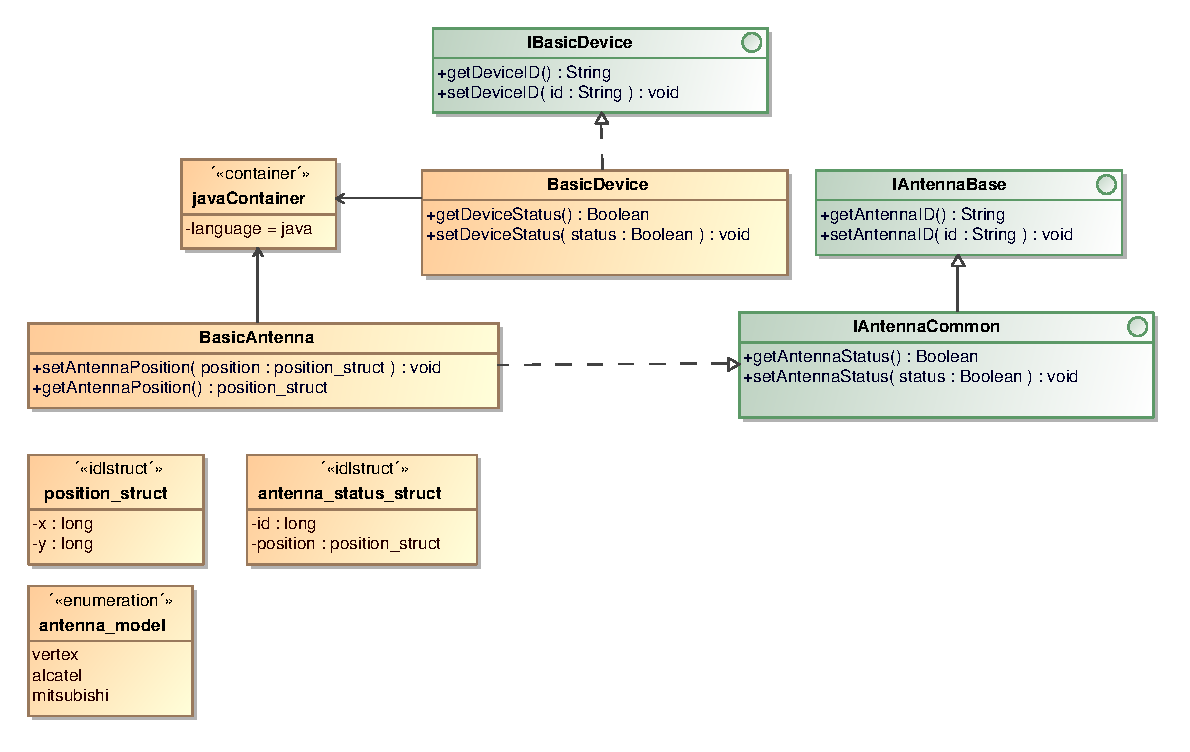
\includegraphics[scale=0.8]{images/example3}
\caption{\label{fig:vs_diag}Interfaces.}
\end{center}
\end{figure*}
\\
In the figure above, the class  \verb+BasicAntenna+ implements the Interface
\verb+IAntennaCommon+ and \verb+IAntennaCommon+ is extended from
\verb+IAntennaBase+, the generator also can implement the inheritance in
Interfaces. The code generated for the \verb+BasicAntenna+ component implements
the all the methods of all  implemented interfaces, if the interface is extended
in one or multiple levels, the generator implements all methods of the interface
inheritance (Java OOP constraints) and the IDL file implement this methods to.

Code generated, the component implementes the java interface defined in the
model above.
\begin{center}
\begin{verbatim}
...
public class BasicAntennaBase
      implements
         ComponentLifecycle,
              BasicAntennaBaseOperations,
              IAntennaCommon {
...
\end{verbatim}
\end{center}

And all methods from \verb+IAntennaCommon+, \verb+IAntennaBase+  are implemented
in the component.
\begin{center}
\begin{verbatim}
...
    /*
     * Implements the Interface methods.
     */
    @Override
    public boolean getAntennaStatus() {...

    @Override
    public void setAntennaStatus(boolean status) {...

    @Override
    public String getAntennaID() {...

    @Override
    public void setAntennaID(String id) {....
 ...
\end{verbatim}
\end{center}

Also the IDL file of the component is implemented with this methods to:
\begin{center}
\begin{verbatim}
...
#ifndef BasicAntenna_IDL
#define BasicAntenna_IDL
#include <acscomponent.idl>
#include <example3Common.idl>

#pragma prefix "alma"

module example3
{
    interface BasicAntennaBase : ACS::ACSComponent
    {
        void setAntennaPosition(in position_struct position);
        position_struct getAntennaPosition();
        boolean getAntennaStatus();
        void setAntennaStatus(in boolean status);
        string getAntennaID();
        void setAntennaID(in string id);
    };
};
#endif /* example3_IDL */
...
\end{verbatim}
\end{center}

This example can be downloaded from:
http://acsccg.googlecode.com/files/example3.tar.gz

\subsection{Inheritance}

\subsubsection{Multiple Level}
The generator is designed to support inheritance in one ore more inherited
levels, with the ability to override the inherited methods from the parenet, or,
override all methods inherited in all inherited levels.\\
This can be viewed in figure 5.

\begin{figure*}[h!t]
\begin{center}
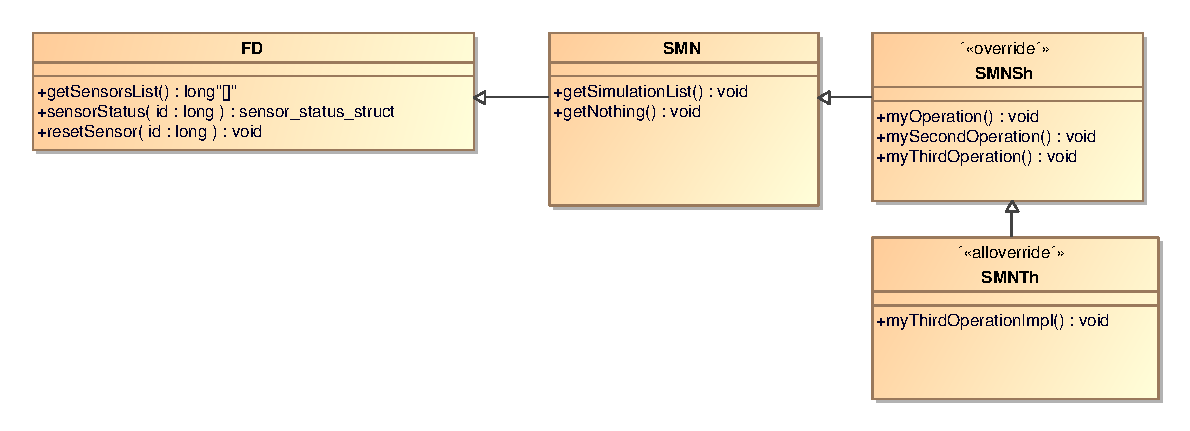
\includegraphics[scale=0.75]{images/simpleinheritance}
\caption{\label{fig:vs_diag}Inheritance in the generator}
\end{center}
\end{figure*}

The class SMN is extended from FD class and inherits implicitly the methods
from FD without override them.\\ 
The class SMNSh is extended from SMN, and override the methods from SMN.\\
The class SMNTh is extended from SMNSh and override all methods inherited, the
methos from FD, SMN and SMNh.\\
\\
A stereotype will differentiate if the class generated must apply the override
policy in the inhertance.

\subsubsubsection{Characteristic Component}
A class with the stereotype \verb+<<Characteristic>>+, if is extended from
other class, the generator will not implement the inheritance in the Java code,
because the Java OOP paradigm not support multiple inheritance (parallel
inheritance) and the class with \verb+<<Characteristic>>+, the generator will
generate the class already extended from ACS class 'CharacteristicComponentImpl'.
 


\newpage

\subsection{Interfaces and Abstract classes}
For desing pattern implementations, the generator support basic features of
Java OOP as Interfaces or Abstract Classes.
\subsubsection{Interface Classes}
The generator support the interface implementation specified in the model and
provides the generated code under the Java OOP standard. It follow the OOP Java
Paradigm.\\
Any class can implemented one or more interfaces, the methods implemented from
the interface will be generated.
An example of this can be viewed in Figure 8.
\begin{figure*}[h!t]
\begin{center}
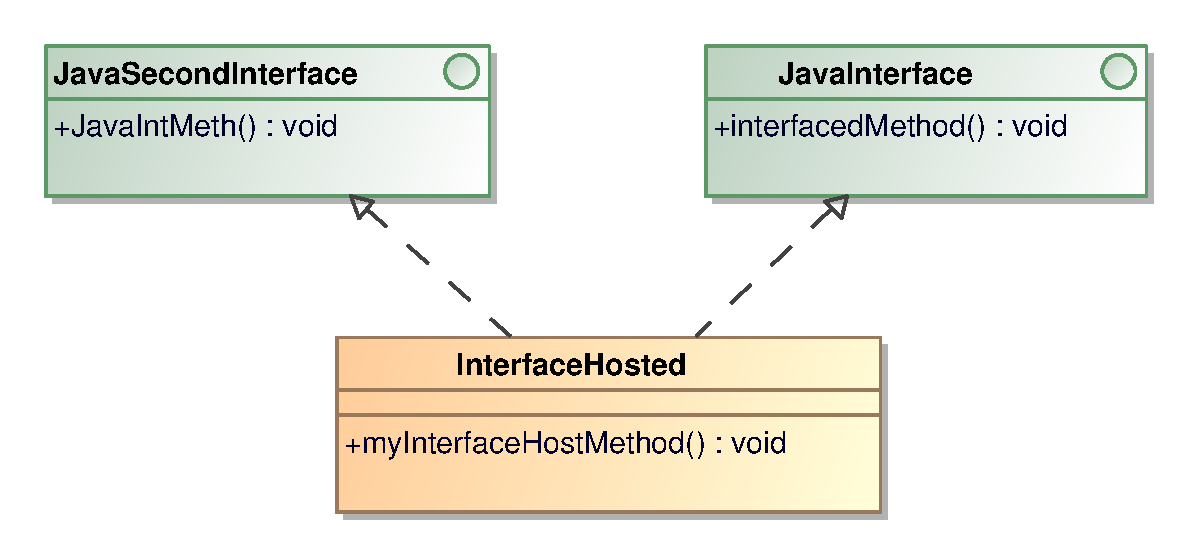
\includegraphics[scale=0.6]{images/interface}
\caption{\label{fig:vs_diag}Interface Example}
\end{center}
\end{figure*}

Will generate :
\begin{verbatim}
public class InterfaceHosted implements ComponentLifecycle,
InterfaceHostedOperations, JavaInterface, JavaSecondInterface {
...
}
\end{verbatim}

\subsubsection{Abstract Classes}
Same as interface implementation, the generator support the abstract class
definition and generate the code.\\
Classes with the \verb+<<Characteristic>>+ stereotype, the generator will no
generate this classes as Abstract.

\subsection{Implemented Code v/s Generated Code}
In every model driven development and code generators, is important how make a
strategy to separate the code already generated with the code implemented over
the generated code.\\
They are three ways solve this.

\subsubsection{EMF Veto Strategy and Inheritance}
The Veto EMF strategy (see Generator Optimization section) is a good solution
using inheritance to implement new things, but, must be create a new class for every change in our code to void
override the whole code already generated, so, this is not the best solution,
but, it works.

\subsubsection{GAP Desing Pattern}
The generation GAP desing pattern provides separate the code with all
hand-modifications implemented in sub-classes, this mean that the core classes
are generated only once and the hand-made implementations, are extended as
subclases from core classes.

\subsubsection{Protected Areas}
Xpand, provides protected areas to our generated code, this mean, that certain
areas with the protected tag with a unique autegenerated ID, can be modified by
the developer without loosing the hand-modifications over the generated code
when the code is re-generated (even if classes are changed in the model).
i.e.: This code went generated with protected areas.
\begin{verbatim}
1. public void getSimulationList() {
2. /*PROTECTED REGION ID(getSimulationList) ENABLED START*/
3.    //Implementation Method here!
4. /*PROTECTED REGION END*/
5. }

1. Method definition
2. Start Protected Area
3. Method hand implementation
4. End Protected Area
\end{verbatim}
Protected areas are specified in generator templates, the generator analize the
generated code, check the code with the template, and protect the area from the
regeneration. If the protected region is not in the templates, the generator
will void the area.\\
In methods, only the implementation is protected and for the code that scape
from UML model every class has a protected area for custom imports, variables and methods.
